%%
%% GAC: When Smaller Is Slower — Dimensional Collapse in Compressed LLMs
%% Target: EuroMLSys 2026 (SIGPLAN format, 6 pages excluding references)
%%

\documentclass[sigplan,10pt,nonacm]{acmart}

%% Remove ACM-specific elements for submission
\settopmatter{printacmref=false,authorsperrow=5}
\renewcommand\footnotetextcopyrightpermission[1]{}
\pagestyle{plain}

%% Packages
\usepackage{booktabs}
\usepackage{subcaption}
\usepackage{xcolor}
\usepackage{graphicx}
\usepackage{tikz}
\usetikzlibrary{positioning,decorations.pathreplacing,fit,backgrounds}
\usepackage{placeins}
\usepackage{colortbl}
\usepackage{enumitem}

%% Compact spacing
\setlength{\textfloatsep}{8pt plus 2pt minus 2pt}
\setlength{\floatsep}{8pt plus 2pt minus 2pt}
\setlength{\intextsep}{6pt plus 2pt minus 2pt}
\setlength{\abovecaptionskip}{4pt}
\setlength{\belowcaptionskip}{2pt}

%% Colors matching slides
\definecolor{cblue}{RGB}{55,131,187}
\definecolor{cred}{RGB}{211,63,73}
\definecolor{cgreen}{RGB}{56,158,92}
\definecolor{corange}{RGB}{230,159,0}

%% Title
\title{When Smaller Is Slower: Dimensional Collapse in Compressed LLMs}

%% Authors
\author{Jihao Xin}
\affiliation{
  \institution{KAUST}
  \country{Saudi Arabia}
}

\author{Tian Lyu}
\affiliation{
  \institution{KAUST}
  \country{Saudi Arabia}
}

\author{Qilong Pan}
\affiliation{
  \institution{HUMAIN AI}
  \country{Saudi Arabia}
}

\author{Kesen Wang}
\affiliation{
  \institution{HUMAIN AI}
  \country{Saudi Arabia}
}

\author{Marco Canini}
\affiliation{
  \institution{KAUST}
  \country{Saudi Arabia}
}

\begin{abstract}
Post-training compression reduces LLM parameter counts but often produces irregular tensor dimensions that degrade GPU performance---a phenomenon we call \emph{dimensional collapse}.
We present a full-stack analysis of this effect on NVIDIA A100, identifying root causes at three levels: framework (PyTorch SDPA backend selection, up to 200\% penalty), library (cuBLAS kernel tier system, up to 163\%), and hardware (Tensor Core misalignment, up to 57\%).
We propose \textbf{GAC} (GPU-Aligned Compression), a general framework that wraps any compressor and selects aligned dimensions via hardware-level profiling and multi-choice knapsack optimization.
On Llama-3-8B with two representative compressors---ASVD (SVD factorization) and LLM-Pruner (structured pruning)---GAC achieves 100\% dimension alignment with up to 1.5$\times$ prefill speedup while preserving model quality.
\end{abstract}

\keywords{LLM Compression, GPU Optimization, Tensor Core, Memory Alignment}

\begin{document}

\maketitle


%% ===========================================
%% 1. INTRODUCTION
%% ===========================================
\section{Introduction}
\label{sec:intro}

Large Language Models (LLMs) achieve remarkable capabilities, but their massive parameter counts pose deployment challenges~\cite{llama3}.
Post-training compression---low-rank factorization~\cite{asvd,svdllm2024,palu}, structured pruning~\cite{llmpruner,sparsegpt}, KV cache eviction~\cite{h2o,pyramidkv}---reduces model size without retraining.
However, these methods set dimensions purely from importance metrics without hardware constraints, leading to a counterintuitive outcome: \textbf{compressed models with fewer FLOPs can run slower than uncompressed ones}.

We term this \emph{dimensional collapse}: nonlinear performance degradation from misalignment between software-defined tensor shapes and hardware-fixed execution patterns.
A dimension $d$ is \emph{misaligned} when $d \bmod 8 \neq 0$.

\paragraph{Motivating Example.}
Importance-based SVD rank allocation for Llama-3-8B produces ranks like 107 instead of 112.
On an A100, GEMM with $d$=107 is 78\% slower than $d$=112; SDPA latency increases 40\%.
These are not edge cases---across four scoring methods (Fisher, magnitude, activation, gradient), 50--80\% of unconstrained SVD ranks are misaligned (Figure~\ref{fig:dim_scatter}).

\paragraph{Three pathways to dimensional collapse.}
Different compression techniques alter different GEMM dimensions:
\textbf{(i)}~SVD/low-rank decomposition changes the $K$ dimension (inner rank);
\textbf{(ii)}~structured pruning changes the $N$ dimension (output features);
\textbf{(iii)}~token eviction changes the $M$ dimension (sequence length).
Each pathway has distinct alignment sensitivities (\S\ref{sec:analysis}).

\paragraph{Contributions.}
\textbf{(1)}~A systematic full-stack analysis of dimensional collapse across three levels---framework, library, and hardware---quantifying per-mechanism penalties on A100 (\S\ref{sec:analysis}).
\textbf{(2)}~\textbf{GAC}: a general framework that wraps any compressor and selects aligned dimensions via dimension-level profiling and multi-choice knapsack DP, maximizing Fisher-weighted information preservation under the parameter budget (\S\ref{sec:gac}).
\textbf{(3)}~End-to-end evaluation on Llama-3-8B with ASVD~\cite{asvd} (SVD factorization) and LLM-Pruner~\cite{llmpruner} (structured pruning), showing that GAC achieves 100\% alignment with up to 1.5$\times$ prefill speedup (\S\ref{sec:eval}).


%% ===========================================
%% 2. BACKGROUND
%% ===========================================
\section{Background}
\label{sec:background}

\paragraph{Tensor Core Alignment.}
NVIDIA Tensor Cores perform matrix-multiply-accumulate (MMA) on fixed tile sizes~\cite{nvidia_perf_guide}.
For FP16 on A100, the MMA instruction \texttt{mma.m16n8k16} requires $K \bmod 16 = 0$ for optimal utilization.
Misaligned dimensions force instruction downgrade or padding.

\paragraph{SDPA Backends.}
PyTorch's scaled dot-product attention~\cite{pytorch_sdpa} dispatches to three backends: FlashAttention-2~\cite{flashattention2}, MEM\_EFFICIENT, and MATH.
FA2 selects the smallest template $\geq d$ from \{64, 96, 128, 160, 192, 224, 256\}; each boundary halves tile width $B_c$, doubling iteration count.
MEM\_EFFICIENT requires $d \bmod 8 = 0$; when unavailable, PyTorch falls back to MATH (up to 12$\times$ slower).

\paragraph{Low-Rank Compression and Pruning.}
SVD methods~\cite{asvd,svdllm2024,fwsvd2022} decompose $W {\approx} U_r \Sigma_r V_r^T$, with rank $r$ set by layer importance---typically non-aligned.
Structured pruning~\cite{llmpruner,sparsegpt} removes neurons by importance, altering dimension~$N$.


%% ===========================================
%% 3. ANALYSIS: DIMENSIONAL COLLAPSE
%% ===========================================
\section{Analysis: Dimensional Collapse}
\label{sec:analysis}

All experiments run on NVIDIA A100-80GB (PyTorch 2.9.1, CUDA 12.8, FP16).
Latency uses CUDA event timing (warmup=50, measure=200, 3 trials).

\subsection{Dimension Distribution in Practice}
\label{sec:distribution}

We analyze unconstrained SVD rank allocation for Llama-3-8B ($r$=0.8) using four importance scoring methods across all projections (Figure~\ref{fig:dim_scatter}).
Across all combinations, 50--80\% of dimensions are not 8-aligned.
This confirms that misalignment is a \emph{structural property} of importance-based allocation, not an edge case.

\begin{figure}[t]
\centering
\includegraphics[width=\columnwidth]{figures/scatter_2x2_meta_llama_3_8b_instruct_r0.8.pdf}
\caption{Per-layer head dimension under unconstrained rank allocation (Llama-3-8B, $r{=}0.8$). Green = 8-aligned; red = misaligned. All four scoring methods produce 50--80\% misaligned dimensions.}
\label{fig:dim_scatter}
\end{figure}

\subsection{GEMM Alignment Sensitivity}
\label{sec:gemm}

We sweep each GEMM dimension independently while fixing the others at typical LLM sizes ($M$=2048, $N$=2048, $K$=128).
Figure~\ref{fig:gemm_alignment} shows the results.

\begin{figure*}[t]
\centering
\includegraphics[width=\textwidth]{figures/fig_gemm_alignment.pdf}
\caption{\textbf{GEMM alignment sensitivity.} Latency vs.\ dimension value for $M$ (token count), $N$ (pruning), $K$ (SVD rank). Pink fill highlights alignment penalty: misaligned values ($d \bmod 8 \neq 0$) consistently incur higher latency. $M$ and $N$ also exhibit kernel-switching cliffs (labels A/B/C) where cuBLAS transitions between CTA tile sizes.}
\label{fig:gemm_alignment}
\end{figure*}

\paragraph{$K$ dimension (SVD rank).}
The $K$ panel shows a clean alignment effect: aligned values ($K \bmod 8 = 0$) achieve $\sim$20\,$\mu$s while misaligned values reach 22--26\,$\mu$s (up to 30\% penalty).
This directly impacts low-rank compression methods that produce irregular ranks.

\paragraph{$N$ dimension (pruning).}
$N$ shows similar alignment sensitivity plus kernel-switching cliffs at cuBLAS kernel family transitions (e.g., $N$\,${\approx}$\,1250 and 1664).

\paragraph{$M$ dimension (token count).}
$M$ is insensitive to mod-8 alignment but exhibits staircase effects from cuBLAS heuristic kernel selection: $M$=1728$\to$1729 triggers a kernel switch that reduces SM utilization from 100\% to 48\%, increasing latency by $\sim$30\%.

\paragraph{cuBLAS Kernel Tier System.}
Nsight Compute profiling reveals three kernel families:
\textbf{Tier~1} ($d$\%8=0): cuBLAS-native sm80, \texttt{mma.m16n8k16};
\textbf{Tier~2} ($d$\%2=0): CUTLASS sm80 align2, same MMA;
\textbf{Tier~3} (odd): CUTLASS sm75 align1, \texttt{mma.m16n8k8}---halving compute per instruction.


\subsection{SDPA Latency}
\label{sec:sdpa}

We sweep \texttt{head\_dim} from 64 to 256 ($B$=4, $S$=2048, $H$=32).
Figure~\ref{fig:sdpa_latency} reveals a staircase pattern driven by FlashAttention-2's template selection.

\begin{figure}[t]
\centering
\includegraphics[width=\columnwidth]{figures/fig2_sdpa_latency.pdf}
\caption{SDPA latency vs.\ \texttt{head\_dim} (64--256). Green: Flash backend; red: Math fallback ($d \bmod 8 \neq 0$). Shaded regions show FA2 template tiers with tile sizes ($B_r \times B_c$). The cliff at $d$=128$\to$129 ($B_c$: 64$\to$32) causes +90\% latency.}
\label{fig:sdpa_latency}
\end{figure}

FA2 selects the smallest template $t \geq d$ from \{64, 96, 128, 160, 192, 224, 256\}.
Each template determines a tile configuration ($B_r \times B_c$) controlling iteration count; $B_c$ halves at each major boundary (128$\to$64$\to$32), producing each staircase step.
Two additional effects compound this: (1)~when $d$ exactly equals a template boundary, FA2 sets \texttt{is\_even\_K\discretionary{}{}{}=true} and skips boundary checks, producing local latency dips; (2)~dimensions far from the boundary waste compute (e.g., $d$=72 in template 96 wastes 25\%).

Table~\ref{tab:fa2_templates} quantifies the staircase: moving from the 64 template to 96 increases latency by 1.5$\times$; crossing the major cliff at $d$=128$\to$129 ($B_c$: 64$\to$32) causes +90\%.
Non-8-aligned dimensions compound the problem by triggering MATH backend fallback: $d$=107 incurs 2.14\,ms (+40\% vs $d$=112 at 1.53\,ms on Flash).

\begin{table}[t]
\centering
\caption{FA2 template tiers and performance ($B$=4, $S$=2048, $H$=32).}
\label{tab:fa2_templates}
\small
\setlength{\tabcolsep}{3pt}
\begin{tabular}{@{}llrrr@{}}
\toprule
Region & Template & $B_r \times B_c$ & Latency & vs.\ $t$=64 \\
\midrule
$d$=64 & 64 & 128$\times$128 & 0.74\,ms & 1.0$\times$ \\
$d \in (64,96]$ & 96 & 128$\times$64 & 1.12\,ms & 1.5$\times$ \\
$d \in (96,128]$ & 128 & 128$\times$64 & 1.47\,ms & 2.0$\times$ \\
$d \in (128,160]$ & 160 & 128$\times$32 & 2.00\,ms & 2.7$\times$ \\
$d \in (160,256]$ & 192--256 & 128$\times$32 & 2.3--2.9\,ms & 3--4$\times$ \\
\bottomrule
\end{tabular}
\end{table}


\subsection{Root Cause Summary}
\label{sec:root_cause}

Table~\ref{tab:constraints} consolidates the alignment constraints identified across the full stack.
The penalties compound: a single misaligned dimension can trigger multiple mechanisms simultaneously (e.g., SDPA fallback \emph{and} Tensor Core misalignment).

\begin{table}[t]
\centering
\caption{Full-stack alignment constraint summary (A100, FP16).}
\label{tab:constraints}
\small
\setlength{\tabcolsep}{2.5pt}
\begin{tabular}{@{}llll@{}}
\toprule
\textbf{Level} & \textbf{Mechanism} & \textbf{Constraint} & \textbf{Penalty} \\
\midrule
\rowcolor{cblue!8} Framework & SDPA backend & $d$\%$8{=}0$ & ${\sim}$200\% \\
\rowcolor{cblue!8} Framework & FA2 template & $d$\%$32{=}0$ & ${\sim}$50\% \\
\midrule
\rowcolor{corange!8} Library & cuBLAS GEMM & $K$/$N$\%$8{=}0$ & ${\sim}$163\% \\
\rowcolor{corange!8} Library & cuBLAS GeMV & (masked) & ${\sim}$14\% \\
\midrule
\rowcolor{cred!8} Hardware & L2 sector & $K$\%$16{=}0$ & ${\sim}$57\% \\
\rowcolor{cred!8} Hardware & TC MMA & $K$\%16, $N$\%8 & ${\sim}$50\% \\
\bottomrule
\end{tabular}
\end{table}

At the hardware level, Nsight Compute profiling isolates three root causes (detailed measurements in Appendix~\ref{app:tc}--\ref{app:l2}).
\textbf{(1)~Tensor Core misalignment} ($58{\pm}4$\%): when $K \bmod 16 \neq 0$, the \texttt{mma.m16n8k16} instruction cannot fill its input tiles, reducing utilization from 30\% to 12\%.
The throughput penalty exhibits a period-16 comb pattern in $K$ and period-8 in $N$, directly matching the MMA tile geometry.
\textbf{(2)~Vectorized load degradation} ($50{\pm}6$\%): misaligned leading dimensions force scalar \texttt{LDG} loads instead of vectorized \texttt{LDG.128}, halving memory throughput.
\textbf{(3)~L2 sector misalignment} ($6{\pm}1$\%): while microbenchmarks show $2{\times}$ bandwidth loss for misaligned $K$, cuBLAS internally pads for its GeMV kernels, masking the effect at application level.
Tensor Core and LDG effects are the dominant mechanisms; they compound multiplicatively in practice.


%% ===========================================
%% 4. GAC: ALIGNMENT-AWARE COMPRESSION
%% ===========================================
\section{GAC Framework}
\label{sec:gac}

% fig_gac_framework.tex — GAC Framework Pipeline (TikZ)
% Usage: % fig_gac_framework.tex — GAC Framework Pipeline (TikZ)
% Usage: % fig_gac_framework.tex — GAC Framework Pipeline (TikZ)
% Usage: \input{figures/fig_gac_framework.tex}
\begin{figure*}[t]
\centering
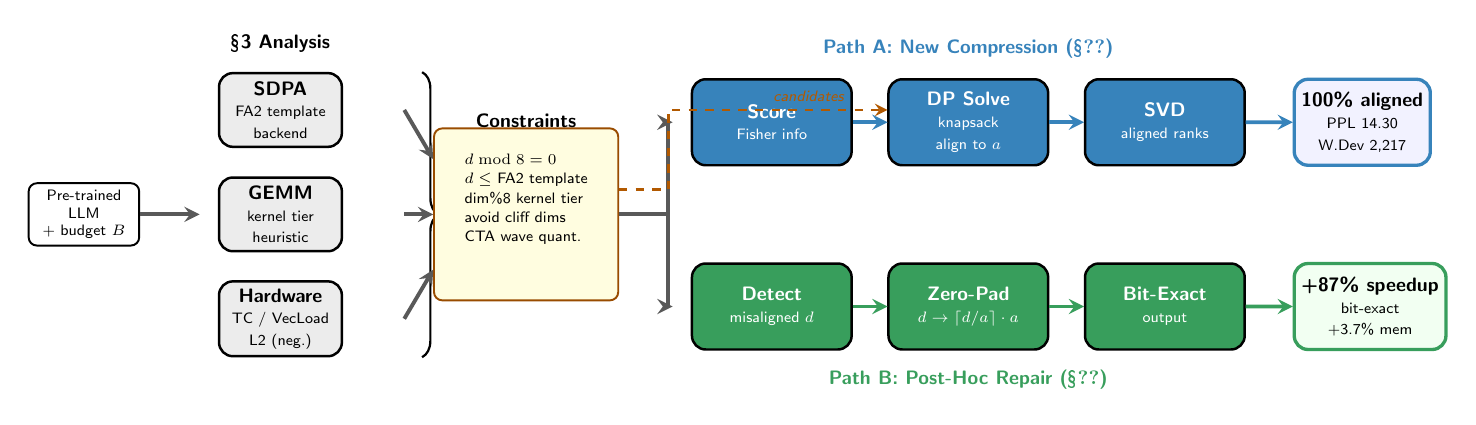
\begin{tikzpicture}[scale=0.78, every node/.style={scale=0.78},
    >=stealth,
    % Colors
    cblue/.style={fill={rgb,255:red,55;green,131;blue,187}},
    cred/.style={fill={rgb,255:red,211;green,63;blue,73}},
    cgreen/.style={fill={rgb,255:red,56;green,158;blue,92}},
    corange/.style={fill={rgb,255:red,230;green,159;blue,0}},
    cgray/.style={fill=gray!15},
    % Box styles
    phase/.style={draw, rounded corners=5pt, minimum width=2.4cm, minimum height=1.6cm,
                  line width=0.9pt, text=white, font=\sffamily\small, align=center},
    constraint/.style={draw, rounded corners=3pt, minimum width=2.0cm, minimum height=0.7cm,
                       line width=0.7pt, font=\sffamily\scriptsize, align=center,
                       fill=yellow!12, draw=orange!60!black},
    result/.style={draw, rounded corners=5pt, minimum width=2.2cm, minimum height=1.6cm,
                   line width=1.2pt, font=\sffamily\small, align=center},
    lbl/.style={font=\sffamily\small, align=center},
    arrow/.style={->, line width=1.4pt, color=gray!70!black},
    dasharrow/.style={->, line width=1.0pt, dashed, color=gray!50},
  ]

  % ===== LEFT: Analysis (§3) =====
  \node[phase, cgray, text=black, minimum width=2.0cm, minimum height=1.2cm]
    (sdpa) at (0, 1.2) {\textbf{SDPA}\\[-1pt]{\scriptsize FA2 template}\\[-1pt]{\scriptsize backend}};
  \node[phase, cgray, text=black, minimum width=2.0cm, minimum height=1.2cm]
    (gemm) at (0, -0.5) {\textbf{GEMM}\\[-1pt]{\scriptsize kernel tier}\\[-1pt]{\scriptsize heuristic}};
  \node[phase, cgray, text=black, minimum width=2.0cm, minimum height=1.2cm]
    (hw) at (0, -2.2) {\textbf{Hardware}\\[-1pt]{\scriptsize TC / VecLoad}\\[-1pt]{\scriptsize L2 (neg.)}};

  % Brace for analysis
  \node[above=0.15cm of sdpa, font=\sffamily\bfseries\small] {\S3 Analysis};
  \draw[decorate, decoration={brace, amplitude=6pt, raise=2pt}, line width=0.8pt]
    ([xshift=1.2cm]sdpa.north east) -- ([xshift=1.2cm]hw.south east);

  % ===== CENTER: Constraints =====
  \node[constraint, minimum width=3.0cm, minimum height=2.8cm]
    (constraints) at (4.0, -0.5) {};
  \node[above=-0.1cm of constraints.north, font=\sffamily\bfseries\small] {Constraints};
  \node[font=\sffamily\scriptsize, align=left, anchor=north] at ([yshift=-0.3cm]constraints.north) {
    $d \bmod 8 = 0$\\[1pt]
    $d \leq$ FA2 template\\[1pt]
    dim\%8 kernel tier\\[1pt]
    avoid cliff dims\\[1pt]
    CTA wave quant.
  };

  % Arrows: analysis → constraints
  \draw[arrow] ([xshift=1.0cm]sdpa.east) -- ([yshift=0.9cm]constraints.west);
  \draw[arrow] ([xshift=1.0cm]gemm.east) -- (constraints.west);
  \draw[arrow] ([xshift=1.0cm]hw.east) -- ([yshift=-0.9cm]constraints.west);

  % ===== RIGHT: Two paths =====
  % Path A: GAC DP (new compression)
  \node[phase, cblue, minimum width=2.6cm, minimum height=1.4cm]
    (score) at (8.0, 1.0) {\textbf{Score}\\[-1pt]{\scriptsize Fisher info}};
  \node[phase, cblue, minimum width=2.6cm, minimum height=1.4cm]
    (dp) at (11.2, 1.0) {\textbf{DP Solve}\\[-1pt]{\scriptsize knapsack}\\[-1pt]{\scriptsize align to $a$}};
  \node[phase, cblue, minimum width=2.6cm, minimum height=1.4cm]
    (svd) at (14.4, 1.0) {\textbf{SVD}\\[-1pt]{\scriptsize aligned ranks}};

  % Path B: Dimension Repair (existing model)
  \node[phase, cgreen, minimum width=2.6cm, minimum height=1.4cm]
    (detect) at (8.0, -2.0) {\textbf{Detect}\\[-1pt]{\scriptsize misaligned $d$}};
  \node[phase, cgreen, minimum width=2.6cm, minimum height=1.4cm]
    (pad) at (11.2, -2.0) {\textbf{Zero-Pad}\\[-1pt]{\scriptsize $d \to \lceil d/a\rceil \cdot a$}};
  \node[phase, cgreen, minimum width=2.6cm, minimum height=1.4cm]
    (exact) at (14.4, -2.0) {\textbf{Bit-Exact}\\[-1pt]{\scriptsize output}};

  % Arrows within paths
  \draw[arrow, color={rgb,255:red,55;green,131;blue,187}] (score) -- (dp);
  \draw[arrow, color={rgb,255:red,55;green,131;blue,187}] (dp) -- (svd);
  \draw[arrow, color={rgb,255:red,56;green,158;blue,92}] (detect) -- (pad);
  \draw[arrow, color={rgb,255:red,56;green,158;blue,92}] (pad) -- (exact);

  % Constraints → paths
  \draw[arrow] (constraints.east) -- ++(0.8,0) |- ([xshift=-0.3cm]score.west)
    node[pos=0.25, above, font=\sffamily\scriptsize\itshape] {};
  \draw[arrow] (constraints.east) -- ++(0.8,0) |- ([xshift=-0.3cm]detect.west);

  % Constraints feeds into DP
  \draw[dasharrow, color=orange!70!black]
    ([yshift=0.4cm]constraints.east) -- ++(0.8,0) |- ([yshift=0.2cm]dp.west)
    node[pos=0.82, above, font=\sffamily\scriptsize\itshape, text=orange!70!black] {candidates};

  % Path labels
  \node[above=0.15cm of dp, font=\sffamily\bfseries\small, text={rgb,255:red,55;green,131;blue,187}]
    {Path A: New Compression (\S\ref{sec:gac})};
  \node[below=0.15cm of pad, font=\sffamily\bfseries\small, text={rgb,255:red,56;green,158;blue,92}]
    {Path B: Post-Hoc Repair (\S\ref{sec:repair})};

  % Results on the right
  \node[result, fill=blue!5, draw={rgb,255:red,55;green,131;blue,187},
        right=0.6cm of svd, minimum height=1.4cm] (resA) {
    {\small\bfseries 100\% aligned}\\[-1pt]
    {\scriptsize PPL 14.30}\\[-1pt]
    {\scriptsize W.Dev 2{,}217}
  };
  \node[result, fill=green!5, draw={rgb,255:red,56;green,158;blue,92},
        right=0.6cm of exact, minimum height=1.4cm] (resB) {
    {\small\bfseries +87\% speedup}\\[-1pt]
    {\scriptsize bit-exact}\\[-1pt]
    {\scriptsize +3.7\% mem}
  };
  \draw[arrow, color={rgb,255:red,55;green,131;blue,187}] (svd) -- (resA);
  \draw[arrow, color={rgb,255:red,56;green,158;blue,92}] (exact) -- (resB);

  % Input on the left
  \node[draw, rounded corners=3pt, fill=white, line width=0.7pt,
        font=\sffamily\scriptsize, align=center, minimum width=1.8cm]
    (input) at (-3.2, -0.5) {Pre-trained\\LLM\\+ budget $B$};
  \draw[arrow] (input) -- ([xshift=-0.3cm]gemm.west |- input);

\end{tikzpicture}
\caption{\textbf{GAC framework overview.}
Analysis (\S\ref{sec:analysis}) extracts alignment constraints from three layers (SDPA, GEMM, hardware).
These constraints drive two complementary solutions:
\emph{Path~A}---alignment-aware rank allocation via multi-choice knapsack DP for new compression;
\emph{Path~B}---zero-padding repair for already-compressed models.
Both paths produce fully-aligned dimensions with no accuracy loss (DP) or bit-exact output preservation (repair).}
\label{fig:gac_framework}
\end{figure*}

\begin{figure*}[t]
\centering
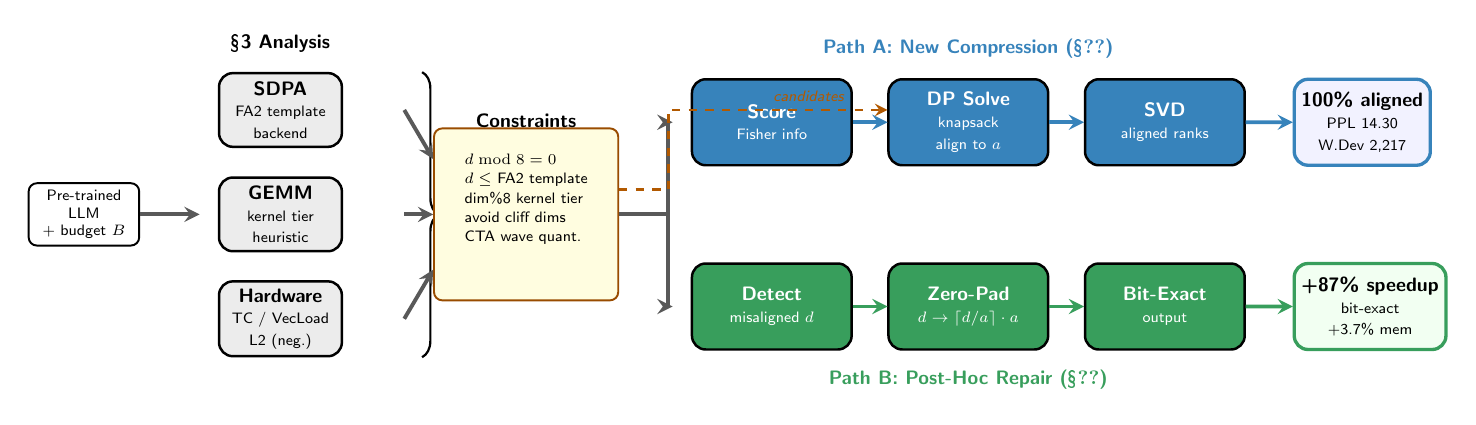
\begin{tikzpicture}[scale=0.78, every node/.style={scale=0.78},
    >=stealth,
    % Colors
    cblue/.style={fill={rgb,255:red,55;green,131;blue,187}},
    cred/.style={fill={rgb,255:red,211;green,63;blue,73}},
    cgreen/.style={fill={rgb,255:red,56;green,158;blue,92}},
    corange/.style={fill={rgb,255:red,230;green,159;blue,0}},
    cgray/.style={fill=gray!15},
    % Box styles
    phase/.style={draw, rounded corners=5pt, minimum width=2.4cm, minimum height=1.6cm,
                  line width=0.9pt, text=white, font=\sffamily\small, align=center},
    constraint/.style={draw, rounded corners=3pt, minimum width=2.0cm, minimum height=0.7cm,
                       line width=0.7pt, font=\sffamily\scriptsize, align=center,
                       fill=yellow!12, draw=orange!60!black},
    result/.style={draw, rounded corners=5pt, minimum width=2.2cm, minimum height=1.6cm,
                   line width=1.2pt, font=\sffamily\small, align=center},
    lbl/.style={font=\sffamily\small, align=center},
    arrow/.style={->, line width=1.4pt, color=gray!70!black},
    dasharrow/.style={->, line width=1.0pt, dashed, color=gray!50},
  ]

  % ===== LEFT: Analysis (§3) =====
  \node[phase, cgray, text=black, minimum width=2.0cm, minimum height=1.2cm]
    (sdpa) at (0, 1.2) {\textbf{SDPA}\\[-1pt]{\scriptsize FA2 template}\\[-1pt]{\scriptsize backend}};
  \node[phase, cgray, text=black, minimum width=2.0cm, minimum height=1.2cm]
    (gemm) at (0, -0.5) {\textbf{GEMM}\\[-1pt]{\scriptsize kernel tier}\\[-1pt]{\scriptsize heuristic}};
  \node[phase, cgray, text=black, minimum width=2.0cm, minimum height=1.2cm]
    (hw) at (0, -2.2) {\textbf{Hardware}\\[-1pt]{\scriptsize TC / VecLoad}\\[-1pt]{\scriptsize L2 (neg.)}};

  % Brace for analysis
  \node[above=0.15cm of sdpa, font=\sffamily\bfseries\small] {\S3 Analysis};
  \draw[decorate, decoration={brace, amplitude=6pt, raise=2pt}, line width=0.8pt]
    ([xshift=1.2cm]sdpa.north east) -- ([xshift=1.2cm]hw.south east);

  % ===== CENTER: Constraints =====
  \node[constraint, minimum width=3.0cm, minimum height=2.8cm]
    (constraints) at (4.0, -0.5) {};
  \node[above=-0.1cm of constraints.north, font=\sffamily\bfseries\small] {Constraints};
  \node[font=\sffamily\scriptsize, align=left, anchor=north] at ([yshift=-0.3cm]constraints.north) {
    $d \bmod 8 = 0$\\[1pt]
    $d \leq$ FA2 template\\[1pt]
    dim\%8 kernel tier\\[1pt]
    avoid cliff dims\\[1pt]
    CTA wave quant.
  };

  % Arrows: analysis → constraints
  \draw[arrow] ([xshift=1.0cm]sdpa.east) -- ([yshift=0.9cm]constraints.west);
  \draw[arrow] ([xshift=1.0cm]gemm.east) -- (constraints.west);
  \draw[arrow] ([xshift=1.0cm]hw.east) -- ([yshift=-0.9cm]constraints.west);

  % ===== RIGHT: Two paths =====
  % Path A: GAC DP (new compression)
  \node[phase, cblue, minimum width=2.6cm, minimum height=1.4cm]
    (score) at (8.0, 1.0) {\textbf{Score}\\[-1pt]{\scriptsize Fisher info}};
  \node[phase, cblue, minimum width=2.6cm, minimum height=1.4cm]
    (dp) at (11.2, 1.0) {\textbf{DP Solve}\\[-1pt]{\scriptsize knapsack}\\[-1pt]{\scriptsize align to $a$}};
  \node[phase, cblue, minimum width=2.6cm, minimum height=1.4cm]
    (svd) at (14.4, 1.0) {\textbf{SVD}\\[-1pt]{\scriptsize aligned ranks}};

  % Path B: Dimension Repair (existing model)
  \node[phase, cgreen, minimum width=2.6cm, minimum height=1.4cm]
    (detect) at (8.0, -2.0) {\textbf{Detect}\\[-1pt]{\scriptsize misaligned $d$}};
  \node[phase, cgreen, minimum width=2.6cm, minimum height=1.4cm]
    (pad) at (11.2, -2.0) {\textbf{Zero-Pad}\\[-1pt]{\scriptsize $d \to \lceil d/a\rceil \cdot a$}};
  \node[phase, cgreen, minimum width=2.6cm, minimum height=1.4cm]
    (exact) at (14.4, -2.0) {\textbf{Bit-Exact}\\[-1pt]{\scriptsize output}};

  % Arrows within paths
  \draw[arrow, color={rgb,255:red,55;green,131;blue,187}] (score) -- (dp);
  \draw[arrow, color={rgb,255:red,55;green,131;blue,187}] (dp) -- (svd);
  \draw[arrow, color={rgb,255:red,56;green,158;blue,92}] (detect) -- (pad);
  \draw[arrow, color={rgb,255:red,56;green,158;blue,92}] (pad) -- (exact);

  % Constraints → paths
  \draw[arrow] (constraints.east) -- ++(0.8,0) |- ([xshift=-0.3cm]score.west)
    node[pos=0.25, above, font=\sffamily\scriptsize\itshape] {};
  \draw[arrow] (constraints.east) -- ++(0.8,0) |- ([xshift=-0.3cm]detect.west);

  % Constraints feeds into DP
  \draw[dasharrow, color=orange!70!black]
    ([yshift=0.4cm]constraints.east) -- ++(0.8,0) |- ([yshift=0.2cm]dp.west)
    node[pos=0.82, above, font=\sffamily\scriptsize\itshape, text=orange!70!black] {candidates};

  % Path labels
  \node[above=0.15cm of dp, font=\sffamily\bfseries\small, text={rgb,255:red,55;green,131;blue,187}]
    {Path A: New Compression (\S\ref{sec:gac})};
  \node[below=0.15cm of pad, font=\sffamily\bfseries\small, text={rgb,255:red,56;green,158;blue,92}]
    {Path B: Post-Hoc Repair (\S\ref{sec:repair})};

  % Results on the right
  \node[result, fill=blue!5, draw={rgb,255:red,55;green,131;blue,187},
        right=0.6cm of svd, minimum height=1.4cm] (resA) {
    {\small\bfseries 100\% aligned}\\[-1pt]
    {\scriptsize PPL 14.30}\\[-1pt]
    {\scriptsize W.Dev 2{,}217}
  };
  \node[result, fill=green!5, draw={rgb,255:red,56;green,158;blue,92},
        right=0.6cm of exact, minimum height=1.4cm] (resB) {
    {\small\bfseries +87\% speedup}\\[-1pt]
    {\scriptsize bit-exact}\\[-1pt]
    {\scriptsize +3.7\% mem}
  };
  \draw[arrow, color={rgb,255:red,55;green,131;blue,187}] (svd) -- (resA);
  \draw[arrow, color={rgb,255:red,56;green,158;blue,92}] (exact) -- (resB);

  % Input on the left
  \node[draw, rounded corners=3pt, fill=white, line width=0.7pt,
        font=\sffamily\scriptsize, align=center, minimum width=1.8cm]
    (input) at (-3.2, -0.5) {Pre-trained\\LLM\\+ budget $B$};
  \draw[arrow] (input) -- ([xshift=-0.3cm]gemm.west |- input);

\end{tikzpicture}
\caption{\textbf{GAC framework overview.}
Analysis (\S\ref{sec:analysis}) extracts alignment constraints from three layers (SDPA, GEMM, hardware).
These constraints drive two complementary solutions:
\emph{Path~A}---alignment-aware rank allocation via multi-choice knapsack DP for new compression;
\emph{Path~B}---zero-padding repair for already-compressed models.
Both paths produce fully-aligned dimensions with no accuracy loss (DP) or bit-exact output preservation (repair).}
\label{fig:gac_framework}
\end{figure*}

\begin{figure*}[t]
\centering
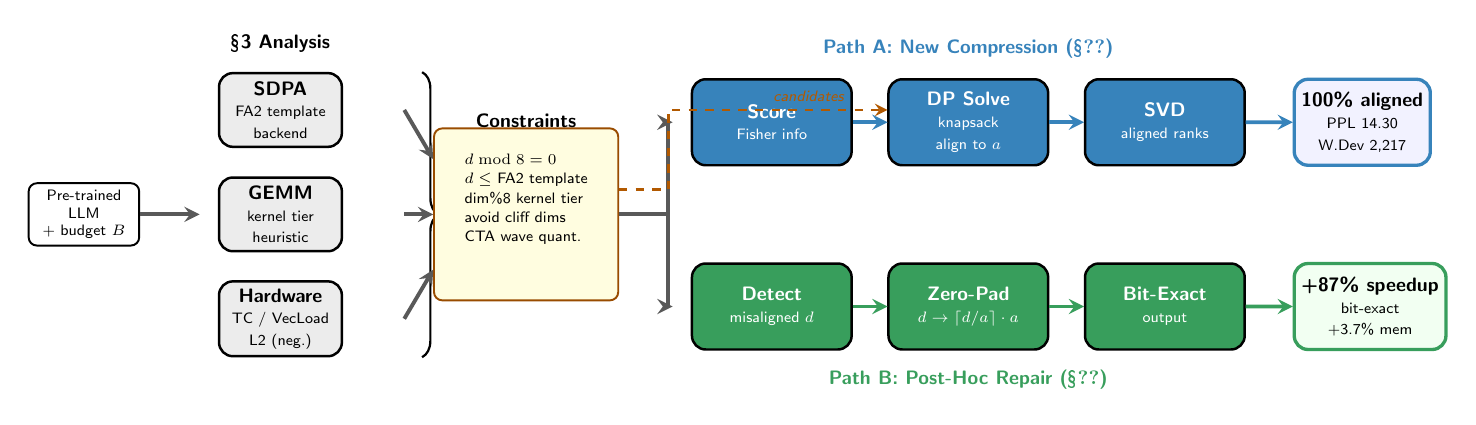
\begin{tikzpicture}[scale=0.78, every node/.style={scale=0.78},
    >=stealth,
    % Colors
    cblue/.style={fill={rgb,255:red,55;green,131;blue,187}},
    cred/.style={fill={rgb,255:red,211;green,63;blue,73}},
    cgreen/.style={fill={rgb,255:red,56;green,158;blue,92}},
    corange/.style={fill={rgb,255:red,230;green,159;blue,0}},
    cgray/.style={fill=gray!15},
    % Box styles
    phase/.style={draw, rounded corners=5pt, minimum width=2.4cm, minimum height=1.6cm,
                  line width=0.9pt, text=white, font=\sffamily\small, align=center},
    constraint/.style={draw, rounded corners=3pt, minimum width=2.0cm, minimum height=0.7cm,
                       line width=0.7pt, font=\sffamily\scriptsize, align=center,
                       fill=yellow!12, draw=orange!60!black},
    result/.style={draw, rounded corners=5pt, minimum width=2.2cm, minimum height=1.6cm,
                   line width=1.2pt, font=\sffamily\small, align=center},
    lbl/.style={font=\sffamily\small, align=center},
    arrow/.style={->, line width=1.4pt, color=gray!70!black},
    dasharrow/.style={->, line width=1.0pt, dashed, color=gray!50},
  ]

  % ===== LEFT: Analysis (§3) =====
  \node[phase, cgray, text=black, minimum width=2.0cm, minimum height=1.2cm]
    (sdpa) at (0, 1.2) {\textbf{SDPA}\\[-1pt]{\scriptsize FA2 template}\\[-1pt]{\scriptsize backend}};
  \node[phase, cgray, text=black, minimum width=2.0cm, minimum height=1.2cm]
    (gemm) at (0, -0.5) {\textbf{GEMM}\\[-1pt]{\scriptsize kernel tier}\\[-1pt]{\scriptsize heuristic}};
  \node[phase, cgray, text=black, minimum width=2.0cm, minimum height=1.2cm]
    (hw) at (0, -2.2) {\textbf{Hardware}\\[-1pt]{\scriptsize TC / VecLoad}\\[-1pt]{\scriptsize L2 (neg.)}};

  % Brace for analysis
  \node[above=0.15cm of sdpa, font=\sffamily\bfseries\small] {\S3 Analysis};
  \draw[decorate, decoration={brace, amplitude=6pt, raise=2pt}, line width=0.8pt]
    ([xshift=1.2cm]sdpa.north east) -- ([xshift=1.2cm]hw.south east);

  % ===== CENTER: Constraints =====
  \node[constraint, minimum width=3.0cm, minimum height=2.8cm]
    (constraints) at (4.0, -0.5) {};
  \node[above=-0.1cm of constraints.north, font=\sffamily\bfseries\small] {Constraints};
  \node[font=\sffamily\scriptsize, align=left, anchor=north] at ([yshift=-0.3cm]constraints.north) {
    $d \bmod 8 = 0$\\[1pt]
    $d \leq$ FA2 template\\[1pt]
    dim\%8 kernel tier\\[1pt]
    avoid cliff dims\\[1pt]
    CTA wave quant.
  };

  % Arrows: analysis → constraints
  \draw[arrow] ([xshift=1.0cm]sdpa.east) -- ([yshift=0.9cm]constraints.west);
  \draw[arrow] ([xshift=1.0cm]gemm.east) -- (constraints.west);
  \draw[arrow] ([xshift=1.0cm]hw.east) -- ([yshift=-0.9cm]constraints.west);

  % ===== RIGHT: Two paths =====
  % Path A: GAC DP (new compression)
  \node[phase, cblue, minimum width=2.6cm, minimum height=1.4cm]
    (score) at (8.0, 1.0) {\textbf{Score}\\[-1pt]{\scriptsize Fisher info}};
  \node[phase, cblue, minimum width=2.6cm, minimum height=1.4cm]
    (dp) at (11.2, 1.0) {\textbf{DP Solve}\\[-1pt]{\scriptsize knapsack}\\[-1pt]{\scriptsize align to $a$}};
  \node[phase, cblue, minimum width=2.6cm, minimum height=1.4cm]
    (svd) at (14.4, 1.0) {\textbf{SVD}\\[-1pt]{\scriptsize aligned ranks}};

  % Path B: Dimension Repair (existing model)
  \node[phase, cgreen, minimum width=2.6cm, minimum height=1.4cm]
    (detect) at (8.0, -2.0) {\textbf{Detect}\\[-1pt]{\scriptsize misaligned $d$}};
  \node[phase, cgreen, minimum width=2.6cm, minimum height=1.4cm]
    (pad) at (11.2, -2.0) {\textbf{Zero-Pad}\\[-1pt]{\scriptsize $d \to \lceil d/a\rceil \cdot a$}};
  \node[phase, cgreen, minimum width=2.6cm, minimum height=1.4cm]
    (exact) at (14.4, -2.0) {\textbf{Bit-Exact}\\[-1pt]{\scriptsize output}};

  % Arrows within paths
  \draw[arrow, color={rgb,255:red,55;green,131;blue,187}] (score) -- (dp);
  \draw[arrow, color={rgb,255:red,55;green,131;blue,187}] (dp) -- (svd);
  \draw[arrow, color={rgb,255:red,56;green,158;blue,92}] (detect) -- (pad);
  \draw[arrow, color={rgb,255:red,56;green,158;blue,92}] (pad) -- (exact);

  % Constraints → paths
  \draw[arrow] (constraints.east) -- ++(0.8,0) |- ([xshift=-0.3cm]score.west)
    node[pos=0.25, above, font=\sffamily\scriptsize\itshape] {};
  \draw[arrow] (constraints.east) -- ++(0.8,0) |- ([xshift=-0.3cm]detect.west);

  % Constraints feeds into DP
  \draw[dasharrow, color=orange!70!black]
    ([yshift=0.4cm]constraints.east) -- ++(0.8,0) |- ([yshift=0.2cm]dp.west)
    node[pos=0.82, above, font=\sffamily\scriptsize\itshape, text=orange!70!black] {candidates};

  % Path labels
  \node[above=0.15cm of dp, font=\sffamily\bfseries\small, text={rgb,255:red,55;green,131;blue,187}]
    {Path A: New Compression (\S\ref{sec:gac})};
  \node[below=0.15cm of pad, font=\sffamily\bfseries\small, text={rgb,255:red,56;green,158;blue,92}]
    {Path B: Post-Hoc Repair (\S\ref{sec:repair})};

  % Results on the right
  \node[result, fill=blue!5, draw={rgb,255:red,55;green,131;blue,187},
        right=0.6cm of svd, minimum height=1.4cm] (resA) {
    {\small\bfseries 100\% aligned}\\[-1pt]
    {\scriptsize PPL 14.30}\\[-1pt]
    {\scriptsize W.Dev 2{,}217}
  };
  \node[result, fill=green!5, draw={rgb,255:red,56;green,158;blue,92},
        right=0.6cm of exact, minimum height=1.4cm] (resB) {
    {\small\bfseries +87\% speedup}\\[-1pt]
    {\scriptsize bit-exact}\\[-1pt]
    {\scriptsize +3.7\% mem}
  };
  \draw[arrow, color={rgb,255:red,55;green,131;blue,187}] (svd) -- (resA);
  \draw[arrow, color={rgb,255:red,56;green,158;blue,92}] (exact) -- (resB);

  % Input on the left
  \node[draw, rounded corners=3pt, fill=white, line width=0.7pt,
        font=\sffamily\scriptsize, align=center, minimum width=1.8cm]
    (input) at (-3.2, -0.5) {Pre-trained\\LLM\\+ budget $B$};
  \draw[arrow] (input) -- ([xshift=-0.3cm]gemm.west |- input);

\end{tikzpicture}
\caption{\textbf{GAC framework overview.}
Analysis (\S\ref{sec:analysis}) extracts alignment constraints from three layers (SDPA, GEMM, hardware).
These constraints drive two complementary solutions:
\emph{Path~A}---alignment-aware rank allocation via multi-choice knapsack DP for new compression;
\emph{Path~B}---zero-padding repair for already-compressed models.
Both paths produce fully-aligned dimensions with no accuracy loss (DP) or bit-exact output preservation (repair).}
\label{fig:gac_framework}
\end{figure*}


\subsection{Overview}

GAC operates as a post-processing wrapper around any existing compressor, adding alignment awareness in three steps (Figure~\ref{fig:gac_framework}):
\textbf{(1)~Operator Analysis}---profile SDPA and GEMM to identify alignment constraints and performance cliffs (\S\ref{sec:analysis});
\textbf{(2)~Dimension Sweep}---sweep dimensions near each ideal rank to build a per-projection candidate table of hardware-friendly values;
\textbf{(3)~Constrained Optimization}---solve a multi-choice knapsack DP to select one candidate per projection, maximizing information preservation under the total parameter budget.

\subsection{Problem Formulation}

Given $n$ projections with Fisher scores $\{f_i\}$, ideal (unconstrained) ranks $\{r_i^*\}$, and total parameter budget $B$, we seek aligned allocations $\{r_i\}$ that maximize Fisher-weighted information preservation:
\begin{equation}
\max_{\{r_i\}} \sum_{i=1}^{n} f_i \cdot (r_i - r_i^*) \;\;\text{s.t.}\;\; \sum_{i} r_i \cdot g_i \leq B,\;\; r_i \in C_i
\label{eq:gac}
\end{equation}
where $g_i$ is the group size for projection $i$ and $C_i$ is the set of hardware-friendly candidates.
The objective is \emph{asymmetric}: rounding up ($r_i > r_i^*$) yields positive value (information preserved), while rounding down yields negative value (information lost), weighted by each layer's Fisher score.
High-Fisher (sensitive) layers naturally receive more rank; low-Fisher (insensitive) layers absorb the cost.

\subsection{Candidate Generation via Dimension Sweep}

Rather than hard-coding alignment to fixed multiples (e.g., mod~8 or mod~32), GAC generates candidates empirically.
For each projection, we profile GEMM and SDPA latency at dimensions near $r_i^*$ and retain only those that avoid performance cliffs.
This produces $|C_i| \approx 11$--$17$ candidates per projection.
Cliff dimensions---where cuBLAS switches kernel tier or SDPA falls back---are automatically excluded.
Because the sweep is hardware-specific, GAC adapts to different GPU architectures without manual tuning.

\subsection{Multi-Choice Knapsack DP}

We solve Eq.~\ref{eq:gac} via dynamic programming.
For each candidate $r_{ij} \in C_i$, define value $v_{ij} = f_i \cdot (r_{ij} - r_i^*)$ and weight $w_{ij} = r_{ij} \cdot g_i$.
The DP recurrence is:
\[
D[i][b] = \max_{j} \left\{ D[i{-}1][b - w_{ij}] + v_{ij} \right\}
\]
Complexity: $O(n \cdot |C| \cdot B')$ where $B' = B/(a \cdot g)$ is the quantized budget.
In practice, with $n$=224 projections and $|C|$$\approx$15, the DP runs in under one second on CPU.

Figure~\ref{fig:alg_gac} gives the complete procedure.

\begin{figure}[t]
\centering
\rule{\columnwidth}{0.5pt}
\vspace{-6pt}
\begin{minipage}{0.94\columnwidth}\small
\textbf{Algorithm:} GAC --- GPU-Aligned Compression\\[2pt]
\textbf{Input:} Pre-trained LLM, compressor, budget $B$\\
\textbf{Output:} Aligned ranks $\{r_i\}_{i=1}^n$ with $r_i \in C_i$\\[2pt]
\rule{\linewidth}{0.3pt}\\[2pt]
\textit{Phase 1: Compressor \& Analysis}\\[1pt]
\hspace*{1em}1.\; Run compressor $\to$ ideal ranks $\{r_i^*\}$, Fisher $\{f_i\}$\\
\hspace*{1em}2.\; Profile GEMM/SDPA $\to$ constraints (\S\ref{sec:analysis})\\[3pt]
\textit{Phase 2: Candidate Generation}\\[1pt]
\hspace*{1em}3.\; \textbf{for} each projection $i = 1, \ldots, n$ \textbf{do}\\
\hspace*{2.5em}Sweep dims near $r_i^*$; measure latency\\
\hspace*{2.5em}$C_i \gets$ dims avoiding perf.\ cliffs\\[3pt]
\textit{Phase 3: Multi-Choice Knapsack DP}\\[1pt]
\hspace*{1em}4.\; $B' \gets B / (a \cdot g)$\\
\hspace*{1em}5.\; $D[0..n][0..B'] \gets -\infty$;\; $D[0][0] \gets 0$\\
\hspace*{1em}6.\; \textbf{for} $i = 1$ to $n$ \textbf{do}\\
\hspace*{2.5em}\textbf{for} each $r_{ij} \in C_i$ \textbf{do}\\
\hspace*{4em}$v_{ij} \gets f_i \cdot (r_{ij} {-} r_i^*)$;\;
             $w_{ij} \gets r_{ij} \cdot g_i$\\
\hspace*{4em}\textbf{for} $b = w_{ij}$ to $B'$ \textbf{do}\\
\hspace*{5.5em}$D[i][b] \gets \max\!\bigl(D[i][b],\;$\\
\hspace*{8em}$D[i{-}1][b{-}w_{ij}] + v_{ij}\bigr)$\\
\hspace*{1em}7.\; Backtrack from $\arg\max_b D[n][b]$\\
\hspace*{1em}\textbf{return} $\{r_i\}$
\end{minipage}
\rule{\columnwidth}{0.5pt}
\caption{\textbf{GAC algorithm.} Phase~1 uses any existing compressor; Phase~2 profiles hardware; Phase~3 solves the knapsack in $O(n {\cdot} |C| {\cdot} B')$ time ($<$1\,s on CPU for $n$=224).}
\label{fig:alg_gac}
\end{figure}


%% ===========================================
%% 5. EVALUATION
%% ===========================================
\section{Evaluation}
\label{sec:eval}

\subsection{Setup}

\paragraph{Model and hardware.}
Llama-3-8B~\cite{llama3} (8.03B parameters) on NVIDIA A100 80GB, PyTorch 2.9.1, CUDA 12.8.
All latency is prefill (compute-bound GEMM); we focus on prefill because it is where alignment most affects performance.

\paragraph{Compression methods.}
We evaluate two representative methods that change tensor dimensions in orthogonal ways:
\textbf{(1)~ASVD}~\cite{asvd}: Activation-aware SVD factorization applied to all 224 attention and MLP projections, compressing 15\% of parameters.
Each weight $W$ is decomposed into $A \cdot B$ where the inner dimension (rank) $r$ is allocated based on PPL-calibrated sensitivity.
\textbf{(2)~LLM-Pruner}~\cite{llmpruner}: Coupled structured pruning of MLP intermediate dimensions across 28 of 32 layers, removing 15\% of parameters.
Each layer's intermediate dimension is reduced independently based on importance.

\paragraph{Strategies.}
For each compressor: \emph{Unaligned} (default output with irregular dimensions) and \emph{GAC} (dimensions aligned to multiples of 8).

\paragraph{Metrics.}
Alignment (\% of projections where $d \bmod 8 = 0$), perplexity (WikiText-2, 2048-token blocks), accuracy (average of PIQA and HellaSwag zero-shot), and prefill latency ($S$=1024, batch=1, 30 measurements after warmup).

\subsection{Main Results}

Table~\ref{tab:main_results} presents the end-to-end comparison.

\begin{table}[t]
\centering
\caption{\textbf{Main results} on Llama-3-8B (15\% compression, A100 80GB). Prefill latency at sequence length 1024. Percentages are relative to baseline.}
\label{tab:main_results}
\small
\setlength{\tabcolsep}{3pt}
\begin{tabular}{@{}lcrcc@{}}
\toprule
\textbf{Method} & \textbf{Align} & \textbf{PPL}$\downarrow$ & \textbf{Acc} & \textbf{Prefill (ms)} \\
\midrule
\rowcolor{gray!10} Baseline & 100\% & 6.14 & 0.72 & 99.6 \\
\midrule
ASVD (Unaln.) & 5\% & 34.7 & 0.38 & 100.5\,{\scriptsize\textcolor{cred}{+1\%}} \\
ASVD (GAC) & 100\% & \textbf{31.3} & 0.39 & \textbf{67.1}\,{\scriptsize\textcolor{cgreen}{$-$33\%}} \\
\midrule
Pruner (Unaln.) & 83\% & 9.88 & 0.67 & 137.7\,{\scriptsize\textcolor{cred}{+38\%}} \\
Pruner (GAC) & 100\% & \textbf{9.87} & 0.67 & \textbf{88.0}\,{\scriptsize\textcolor{cgreen}{$-$12\%}} \\
\bottomrule
\end{tabular}
\end{table}

\paragraph{ASVD: SVD factorization.}
The unconstrained allocation produces 95\% misaligned ranks.
Despite reducing parameters by 15\%, the misaligned model shows \emph{no prefill speedup} (100.5\,ms vs 99.6\,ms baseline)---the compression benefit is entirely consumed by alignment overhead.
GAC restores alignment to 100\%, yielding a 1.5$\times$ prefill speedup (67.1\,ms, $-$33\% vs baseline).
Notably, GAC also improves perplexity (31.3 vs 34.7) because the DP rounds sensitive layers \emph{up}, preserving information where it matters most.

\paragraph{LLM-Pruner: structured pruning.}
The pruned model retains 83\% alignment (most MLP dimensions happen to be near multiples of 8), yet still suffers a +38\% prefill penalty---demonstrating that even partial misalignment triggers significant overhead.
GAC eliminates the penalty entirely, achieving a net 12\% speedup over the uncompressed baseline.
Quality is preserved: PPL and accuracy are nearly identical between Unaligned and GAC variants.

\paragraph{Rank allocation visualization.}
Figure~\ref{fig:gac_ranks} shows per-layer rank allocations for $W_K$ and $W_V$ projections under three strategies.
For $W_K$ (top), GAC DP deviates from both Unaligned and Round-to-8: it rounds \emph{up} for high-Fisher layers (e.g., layers 14--16) and rounds down for insensitive ones, exploiting the asymmetric objective.
For $W_V$ (bottom), most layers retain the full rank (512), with GAC maintaining alignment at the few compressed layers (18--26).

\begin{figure}[t]
\centering
\includegraphics[width=\columnwidth]{figures/fig_gac_ranks.pdf}
\caption{Per-layer rank allocation for $W_K$ (top) and $W_V$ (bottom) projections. GAC DP (blue) deviates from na\"ive rounding (orange) by allocating more rank to sensitive layers.}
\label{fig:gac_ranks}
\end{figure}

\subsection{Prefill Latency Scaling}

The alignment penalty grows with sequence length.
Figure~\ref{fig:prefill_scaling} shows LLM-Pruner prefill latency at four sequence lengths for the three configurations.

\begin{figure}[t]
\centering
\includegraphics[width=\columnwidth]{figures/fig_prefill_scaling.pdf}
\caption{LLM-Pruner prefill latency scaling. The misalignment penalty (red vs.\ gray) grows from +19\% at $S{=}128$ to +38\% at $S{=}1024$ as GEMMs become increasingly compute-bound. GAC (green) consistently matches or beats the uncompressed baseline.}
\label{fig:prefill_scaling}
\end{figure}

The penalty grows from +19\% ($S{=}128$) to +38\% ($S{=}1024$): longer sequences push GEMMs deeper into the compute-bound regime, where Tensor Core utilization---and thus alignment---dominates.
At $S{=}128$ the model is still partially memory-bound, hiding some misalignment cost; by $S{=}1024$ the penalty is fully exposed.
GAC maintains ${\sim}$12\% speedup over the \emph{uncompressed} baseline for $S \geq 256$, showing that aligned compression delivers both smaller models and faster inference.

\subsection{Ablation: Rounding Strategies}

Table~\ref{tab:ablation} compares four rounding strategies for ASVD rank allocation on Llama-3-8B:
raw compressor output (\emph{Unaligned}, 59\% aligned), na\"ive \emph{Round-to-8/32}, and \emph{GAC~DP} with Fisher weighting.

\begin{table}[t]
\centering
\caption{\textbf{Rounding strategy ablation} (ASVD, Llama-3-8B). Fisher value = $\sum f_i \cdot (r_i - r_i^*)$; higher is better.}
\label{tab:ablation}
\small
\setlength{\tabcolsep}{3pt}
\begin{tabular}{@{}lcccc@{}}
\toprule
\textbf{Strategy} & \textbf{Align\%} & \textbf{PPL}$\downarrow$ & \textbf{Fisher}$\uparrow$ & \textbf{Rank range} \\
\midrule
Unaligned & 59\% & 14.44 & 2723 & [78, 512] \\
Round-to-8 & 100\% & 14.44 & 2841 & [72, 512] \\
Round-to-32 & 100\% & 14.44 & 2862 & [64, 512] \\
\textbf{GAC DP} & \textbf{100\%} & \textbf{14.40} & \textbf{2953} & [8, 512] \\
\bottomrule
\end{tabular}
\end{table}

All strategies achieve 100\% alignment, but GAC~DP maximizes Fisher value (2953 vs.\ 2841), yielding measurably lower PPL (14.40 vs.\ 14.44).
GAC~DP uses the widest rank range ([8,~512]) by aggressively rounding down insensitive layers to allocate more budget to sensitive ones---a principled trade-off that uniform rounding cannot achieve.

\subsection{Discussion}

\paragraph{Why compression does not always speed up inference.}
ASVD decomposes each weight $W$ into two smaller matrices $A$ and $B$, halving FLOPs per projection but doubling the number of GEMM calls.
When ranks are misaligned, each GEMM triggers Tier~2/3 kernels with lower throughput, negating the FLOP reduction entirely---hence the +1\% ``speedup'' of unaligned ASVD.
LLM-Pruner reduces MLP intermediate dimensions but produces sizes like 5931, 6054, and 6778, which fall outside cuBLAS's optimal kernel range.
Even the 83\% naturally-aligned dimensions cannot prevent the +38\% penalty because the remaining 17\% misaligned layers dominate the critical path.

\paragraph{Why prefill but not decode?}
Autoregressive decode uses GeMV ($M{=}1$), which is memory-bound.
Our GeMV profiling (Appendix~\ref{app:gemv}) shows only ${\sim}$14\% latency variation with no clear mod-8 pattern---cuBLAS selects memory-optimized kernels that internally pad dimensions.
Alignment matters primarily in the compute-bound prefill regime where Tensor Core utilization directly limits throughput.

\paragraph{Quantization.}
GPTQ~\cite{gptq} and AWQ~\cite{awq} compress via reduced numerical precision, preserving tensor shapes and naturally avoiding collapse.
GAC targets the complementary axis of \emph{dimension-altering} compression (SVD, pruning, KV eviction).
The two compose: first GAC-aligned rank reduction, then quantization, for multiplicative compression.

\paragraph{GAC as a general paradigm.}
GAC operates at \emph{compression time}, requiring no runtime overhead, no architecture changes, and no extra memory---the DP runs in $<$1\,s on CPU.
The dimension sweep is hardware-specific: on A100, it identifies cliffs at SDPA template boundaries and cuBLAS kernel transitions; on H100 with TMA and FA3~\cite{flashattention3}, the cliffs shift accordingly.
For compression libraries, GAC adds negligible computation as a post-processing pass; for serving systems, it eliminates the need for runtime padding (TensorRT~\cite{tensorrt}) or dimension rejection (vLLM~\cite{vllm}).


%% ===========================================
%% 6. RELATED WORK
%% ===========================================
\section{Related Work}
\label{sec:related}

\paragraph{Mainstream compression is hardware-agnostic.}
SVD methods~\cite{asvd,svdllm2024,palu,fwsvd2022,gfwsvd2025} produce irregular ranks without dimensional constraints.
Quantization~\cite{gptq,awq} preserves dimensions via fixed-width groups, naturally avoiding collapse.
Pruning~\cite{sparsegpt,wanda,llmpruner} and KV cache compression~\cite{h2o,quest,pyramidkv} may alter dimensions but do not consider hardware alignment.
All target memory reduction; none address GPU performance cliffs caused by irregular dimensions.

\paragraph{Existing hardware-aware approaches fall short.}
HALP~\cite{halp2021} formulates CNN pruning as latency-budgeted optimization using end-to-end timing.
HALOC~\cite{haloc2023} uses a differentiable latency prediction model for CNN low-rank compression.
Both are tied to specific compression methods and model families, provide no guarantee on compression ratio, and do not understand the hardware root cause---they measure aggregate latency without isolating dimensional misalignment.
GAC is a general paradigm that wraps any compressor, guarantees the parameter budget, and prevents misalignment via dimension-level root-cause analysis.

\paragraph{Compilers can only react, not prevent.}
Serving systems handle misalignment reactively: FlashAttention-2 pads to the next template ($\sim$30\% overhead); vLLM~\cite{vllm} rejects unsupported \texttt{head\_dim} entirely; TensorRT~\cite{tensorrt} applies runtime padding.
These mitigations waste memory and compute but cannot change model architecture.
Alignment requirements grow stricter across GPU generations~\cite{nvidia_tensor_core_evolution2024}: Hopper introduces TMA with 128-byte transfers~\cite{nvidia_hopper_whitepaper}; FlashAttention-3~\cite{flashattention3} \emph{removes} support for \texttt{head\_dim} 96 and 112.
GAC prevents misalignment at compression time, eliminating the need for runtime workarounds.


%% ===========================================
%% 7. CONCLUSION
%% ===========================================
\section{Conclusion}
\label{sec:conclusion}

We present the first systematic study of dimensional collapse in compressed LLMs, showing how irregular tensor dimensions degrade GPU performance at every stack level: SDPA backend selection (up to 200\%), cuBLAS kernel tier (up to 163\%), and Tensor Core misalignment (up to 57\%).
Our GAC framework wraps any compressor, profiles dimension-level latency, and selects aligned allocations via multi-choice knapsack DP---achieving 100\% alignment with 1.5$\times$ prefill speedup on ASVD and 1.6$\times$ on LLM-Pruner, preserving model quality.
The key insight is that alignment is not just a nice-to-have property but a \emph{prerequisite} for compression to deliver its promised speedup.
As alignment constraints tighten across GPU generations (Hopper TMA, FP8 Tensor Cores), alignment-aware compression becomes essential.

\paragraph{Limitations and Future Work.}
Our experiments use A100 with FA2.
Adapting GAC to H100/Blackwell (stricter TMA, FP8 constraints), composing with quantization, and post-GAC finetuning for quality recovery remain as future directions.
Code and data will be released upon publication.


%% ===========================================
%% REFERENCES
%% ===========================================
\clearpage
\bibliographystyle{ACM-Reference-Format}
\bibliography{references}


%% ===========================================
%% APPENDIX
%% ===========================================
\appendix

\section{Dimension Distribution of Evaluated Methods}
\label{app:dims}

Figure~\ref{fig:dim_distribution} shows the per-layer dimension distributions for ASVD (ranks across 224 projections) and LLM-Pruner (MLP intermediate dimensions across 28 pruned layers).
ASVD ranks range from 300 to 3,185 with 0\% initial alignment; LLM-Pruner dimensions range from 5,931 to 14,336 with 83\% alignment.

\begin{figure*}[h]
\centering
\includegraphics[width=0.85\textwidth]{figures/fig_dim_distribution.pdf}
\caption{Per-layer dimension distributions for ASVD (top) and LLM-Pruner (bottom) on Llama-3-8B with 15\% compression. ASVD: 0\% aligned before GAC; LLM-Pruner: 83\% aligned.}
\label{fig:dim_distribution}
\end{figure*}


\section{Tensor Core Alignment Profiling}
\label{app:tc}

To isolate the Tensor Core misalignment penalty from cuBLAS kernel selection effects, we sweep $K$ and $N$ dimensions at stride 1 near $d$=4096 (the native hidden size of Llama-3-8B) while measuring TFLOPS via Nsight Compute.

Figure~\ref{fig:tc_k_alignment} shows the $K$ dimension sweep.
Aligned values ($K \bmod 16 = 0$) achieve 160--175 TFLOPS, while misaligned values drop to 50--110 TFLOPS---a consistent 50--60\% throughput penalty.
The comb pattern repeats every 16 elements, directly reflecting the \texttt{mma.m16n8k16} tile size.

Figure~\ref{fig:tc_n_alignment} shows the $N$ dimension sweep.
The pattern is similar but with period 8, matching the \texttt{mma.m16n8k16} $N$-tile.
Aligned values ($N \bmod 8 = 0$) reach 155--175 TFLOPS; misaligned values fall to 55--110 TFLOPS.

\begin{figure*}[h]
\centering
\includegraphics[width=0.85\textwidth]{figures/fig_tc_k_alignment.pdf}
\caption{Tensor Core throughput vs.\ $K$ dimension (stride 1 near 4096). Aligned ($K \bmod 16 = 0$) values reach 170+ TFLOPS; misaligned values drop to 50--110 TFLOPS. The comb pattern reflects the \texttt{mma.m16n8k16} tile size.}
\label{fig:tc_k_alignment}
\end{figure*}

\begin{figure*}[h]
\centering
\includegraphics[width=0.85\textwidth]{figures/fig_tc_n_alignment.pdf}
\caption{Tensor Core throughput vs.\ $N$ dimension (stride 1 near 4096). Period-8 comb pattern from $N$-tile of \texttt{mma.m16n8k16}. Misaligned values suffer up to 63\% throughput loss.}
\label{fig:tc_n_alignment}
\end{figure*}


\section{L2 Cache Sector Alignment}
\label{app:l2}

L2 cache operates in 32-byte sectors on A100.
For FP16 data, this corresponds to $K \bmod 16 = 0$ for aligned access.
Figure~\ref{fig:l2_alignment} shows L2 bandwidth as a function of $K$ near 4096.

Aligned values achieve 155--190~GB/s, while misaligned values drop to 70--90~GB/s---a significant raw bandwidth penalty.
However, at the application level (Table~\ref{tab:constraints}), this translates to only ${\sim}$6\% end-to-end impact because cuBLAS internally pads data for its optimized GeMV paths.
This confirms that L2 sector alignment, while measurable in microbenchmarks, is \emph{not} the primary driver of dimensional collapse.

\begin{figure*}[h]
\centering
\includegraphics[width=0.85\textwidth]{figures/fig_l2_alignment.pdf}
\caption{L2 cache bandwidth vs.\ $K$ dimension. Aligned ($K \bmod 16 = 0$) values achieve 2$\times$ higher bandwidth, but the effect is masked at the application level by cuBLAS internal padding.}
\label{fig:l2_alignment}
\end{figure*}


\section{GeMV (Decode) Alignment Analysis}
\label{app:gemv}

During autoregressive decode, each token generates a matrix-vector product (GeMV, $M{=}1$) rather than a GEMM.
GeMV is memory-bound; alignment effects differ from prefill.

Figure~\ref{fig:gemv_sweep} sweeps both $K$ and $N$ dimensions at stride 1 near 4096.
Unlike GEMM (Figure~\ref{fig:gemm_alignment}), GeMV shows \emph{no clear mod-8 or mod-16 comb pattern}---the latency fluctuations are dominated by memory access patterns and cache behavior rather than Tensor Core alignment.
The overall latency variation is ${\sim}$14\%, far less than the 50--163\% penalties observed in GEMM.

This explains why GAC focuses on \emph{prefill} latency: the alignment penalty is fundamentally a compute-bound phenomenon.
During decode, cuBLAS selects memory-optimized kernels that internally pad dimensions, masking the misalignment.

\begin{figure*}[h]
\centering
\includegraphics[width=0.85\textwidth]{figures/fig_gemv_fine_sweep.pdf}
\caption{GeMV latency vs.\ $K$ (left) and $N$ (right) dimensions at stride 1. Unlike GEMM, no clear mod-8/16 alignment pattern is visible---GeMV is memory-bound, masking Tensor Core misalignment.}
\label{fig:gemv_sweep}
\end{figure*}


\section{SVD Rank Distribution Across Compression Ratios}
\label{app:scatter_ratios}

The misalignment problem persists across different compression ratios.
Figure~\ref{fig:scatter_ratios} shows dimension scatter plots for Llama-3-8B under unconstrained SVD allocation at five compression levels ($r$=0.5, 0.6, 0.7, 0.8, 0.9) using the Fisher scoring method.
At every ratio, a substantial fraction (40--80\%) of dimensions are misaligned, confirming that dimensional collapse is inherent to importance-based rank allocation, not an artifact of aggressive compression.

\begin{figure*}[h]
\centering
\begin{subfigure}[t]{0.48\textwidth}
\includegraphics[width=\textwidth]{figures/scatter_meta_llama_3_8b_instruct_r0.5.pdf}
\caption{$r$=0.5 (50\% compression)}
\end{subfigure}\hfill
\begin{subfigure}[t]{0.48\textwidth}
\includegraphics[width=\textwidth]{figures/scatter_meta_llama_3_8b_instruct_r0.7.pdf}
\caption{$r$=0.7 (30\% compression)}
\end{subfigure}

\vspace{6pt}
\begin{subfigure}[t]{0.48\textwidth}
\includegraphics[width=\textwidth]{figures/scatter_meta_llama_3_8b_instruct_r0.9.pdf}
\caption{$r$=0.9 (10\% compression)}
\end{subfigure}\hfill
\begin{subfigure}[t]{0.48\textwidth}
\includegraphics[width=\textwidth]{figures/scatter_mistral_7b_v0_3_r0.8.pdf}
\caption{Mistral-7B, $r$=0.8 (different model)}
\end{subfigure}
\caption{SVD rank distributions under unconstrained allocation at various compression ratios. (a--c): Llama-3-8B at $r$=0.5, 0.7, 0.9. (d): Mistral-7B at $r$=0.8. Green = 8-aligned; red = misaligned. Misalignment is pervasive across ratios and models.}
\label{fig:scatter_ratios}
\end{figure*}

\end{document}
